\documentclass{article}
\usepackage{float}
\usepackage{graphicx}
\usepackage{subfig}
\usepackage{lipsum}
\usepackage{tikz}
\usepackage{eso-pic}
\usepackage{changepage}
\usepackage{xcolor}
\usepackage{afterpage}
\usepackage[document]{ragged2e}
\usepackage[none]{hyphenat}
\usepackage[margin=1in,footskip=0.25in]{geometry}
\usepackage{array}
% \usepackage{l3kernel}
% \usepackage{l3packages}
\usepackage{siunitx}
\usepackage{color,soul}
\usepackage{placeins}
\usepackage{microtype}
\usepackage[backend=biber]{biblatex}
\usepackage[hidelinks]{hyperref}
\usepackage[toc,page]{appendix}
%\usepackage[toc]{glossaries}
\usepackage[subfigure]{tocloft}
\usepackage{rotating}
\usepackage[printwatermark]{xwatermark}
% \usepackage[table,xcdraw]{xcolor}
\usepackage{xcolor}
\hypersetup{
	colorlinks,
	linkcolor={black!50!black},
	citecolor={blue!50!black},
	urlcolor={blue!80!black}
}

\cftsetindents{subsection}{.25in}{.4in}

\usepackage[flushleft]{threeparttable}
\newcolumntype{C}[1]{>{\centering\let\newline\\\arraybackslash\hspace{0pt}}m{#1}}

\definecolor{ULred}{HTML}{872434}

\usepackage{chngcntr}
\counterwithin{table}{section}
\counterwithin{figure}{section}

\pdfoptionpdfminorversion=6
%\addbibresource{FireAttackReport.bib}

\setlength{\parskip}{1em}

% ******* REMOVE COMMENTS AND PLACE GLOSSARY.TEX IN ROOT DIRECTORY TO ADD GLOSSARY, SEE END FOR ADDITIONAL LINES TO UNCOMMENTS *******
%
%\loadglsentries{glossary.tex}
%
%\makeglossaries

% ******* REMOVE COMMENTS ON THIS BLOCK TO ADD DRAFT TO REPORT ********
% \newsavebox\mybox
% \savebox\mybox{\tikz[color=gray,opacity=0.5]\node{DRAFT};}
% \newwatermark*[
% allpages,
% angle=65,
% scale=15,
% xpos=-65,
% ypos=20
% ]{\usebox\mybox}

\begin{document}
	
	\begin{titlepage}
		
		\pagecolor{ULred}\afterpage{\nopagecolor}
		

		\AddToShipoutPictureFG*{\AtPageUpperLeft{\raisebox{-\height}{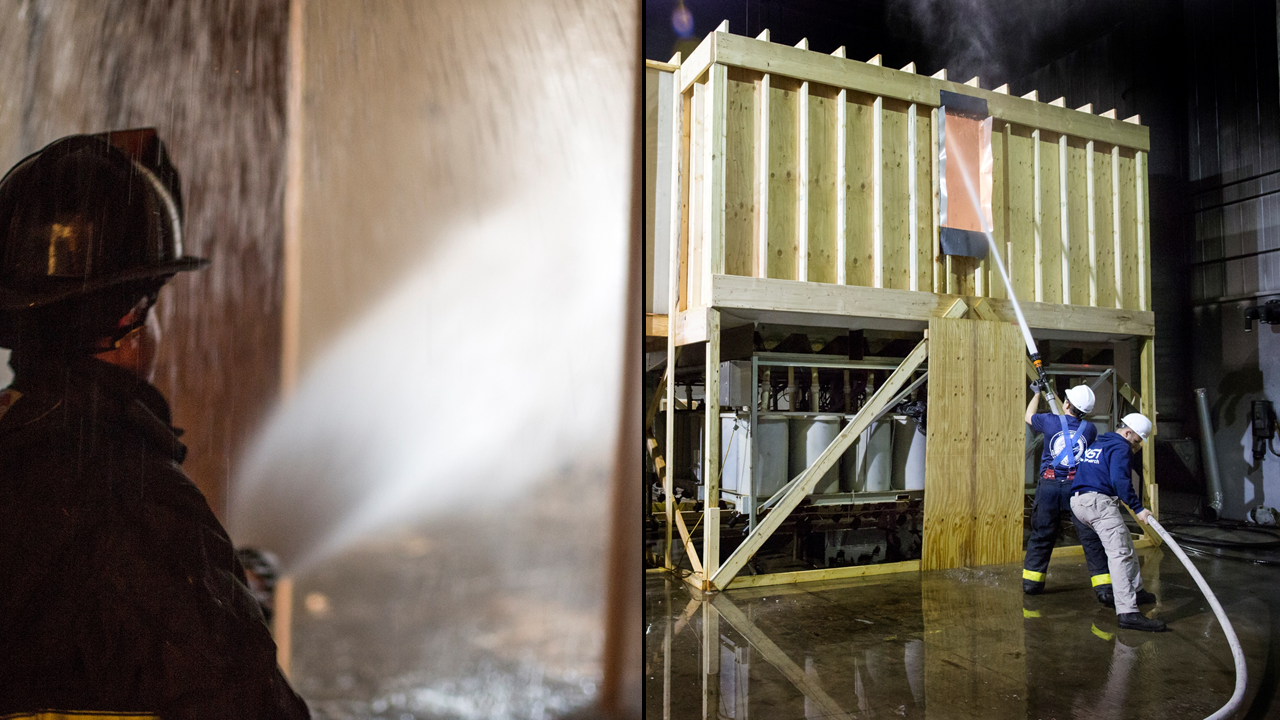
\includegraphics[width=7in]{Figures/General/TitlePagePhoto.png}}}} 

			\vspace*{20\baselineskip} 

		\huge
		\begin{adjustwidth}{-0.5in}{-0in}
		\color{white}
		\textbf{Study of the Impact of Fire Attack \\ Utilizing Interior and Exterior Streams \\ on Firefighter Safety and Occupant Survival}
		\end{adjustwidth}
		\huge
		\begin{adjustwidth}{-0.5in}{-0in}
		\color{white}
		\textbf{Part I: Air Entrainment and Water Distribution}
		\end{adjustwidth}
		\begin{adjustwidth}{-0.5in}{}
		\color{white}
		\vspace{.2\baselineskip}
		\large
		Stephen Kerber \\
		Director \\
		UL Firefighter Safety Research Institute \\
		\vspace*{.5\baselineskip}
		Robin Zevotek \\
		Lead Engineer \\
		UL Firefighter Safety Research Institute \\ 
		\vspace*{.5\baselineskip}
		Keith Stakes \\
		Research Engineer \\
		UL Firefighter Safety Research Institute \\
		\vspace*{.8\baselineskip}	
		\today
		\vspace*{.8\baselineskip}
		\begin{figure}[h]
			\hspace*{-0.5in}
\includegraphics[width=0.75in]{../0_Images/ULLogoWhite.pdf}
		\end{figure}
		\end{adjustwidth}
	\end{titlepage}

\begin{center}
	DISCLAIMER\\
	\vspace*{\baselineskip}
	\begin{adjustwidth}{-0.25in}{-0.25in}
		In no event shall UL be responsible to anyone for whatever use or non-use is made of the information contained in this Report and in no event shall UL, its employees, or its agents incur any obligation or liability for damages including, but not limited to, consequential damage arising out of or in connection  with the use or inability to use the information contained in this Report. Information conveyed by this Report applies only to the specimens actually involved in these tests. UL has not established a factory Follow-Up Service Program to determine the conformance of subsequently produced material, nor has any provision been made to apply any registered mark of UL to such material. The issuance of this Report in no way implies Listing, Classification or Recognition by UL and does not authorize the use of UL Listing, Classification or Recognition Marks or other reference to UL on or in connection with the product or system.
	\end{adjustwidth}
\end{center}

\begin{center}
	FUNDING
\vspace*{\baselineskip}
\begin{adjustwidth}{-0.25in}{-0.25in}
This work was funded through a grant from the Department of Homeland Securities Assistance to Firefighters Grant Program under the Fire Prevention and Safety Grants, Research and Development.
\end{adjustwidth}
\end{center}

\begin{center}
	
\includegraphics[width=0.28\textwidth]{Figures/General/DHS.png}
\end{center}

\clearpage

\renewcommand{\abstractname}{Abstract}
\setlength{\emergencystretch}{5pt}

\begin{abstract}

As research continues into how fire department interventions affect fire dyanmics in the modern fire environment; questions continue to arise on the impact and implications of interior versus exterior fire attack on both firefighter safety and occupant survivability. Previous research into various types of fire ground ventilation, flow paths, and exterior fire streams has provided the fire service with a more in-depth understanding of fire dynamics in addition to raising questions about certain fire attack methods stemming from differing traditions and myths. This knowledge gap and lack of previous research into the impact of fire streams has driven the need for further research into fire department interventions at structure fires with a focus on hose streams and suppression tactics. Statistics show that both firefighters and building occupants continue to loose their lives due to fire. As such, research into the various methods of fire attack will allow a broader understanding of how firefighter interventions on the fire ground can impact the outcome of both life safety and property protection. 

This study will build and expand upon the fire research conducted to date by analyzing how firefighting tactics, specifically suppression methods, affect the thermal exposure and survivability of both firefighters and buidling occupants in addition to impacting fire behavior in structures. The project will be comrprised of 3 parts:
\vspace*{\baselineskip}
\begin{itemize}
	\item Part I: Air Entrainment and Water Distribution.
	\item Part II: Full-scale Residential Fire Experiments.
	\item Part III: Acquired Structure Fire Testing.
	\end{itemize}
\vspace*{\baselineskip}
This report details the experimental data from the air entrainment and water distribution experiments. Results from the first two experiment series were analyzed and reviewed with assistance from our technical panel. These results were summarized into tactical considerations and can be seen below:

\vspace*{\baselineskip}
\noindent \bf{Air Entrainment} -
\normalfont
\begin{itemize}
	\item Air entrainment in nozzles is dependent on nozzle type (smooth bore, straight stream, fog) and not nozzle manufacturer.
	\item Air entrainment in nozzles is dependent on structure geometry and configurations.
	\item Nozzle application patterns have little effect on overall air entrainment.
	\item Air entrainment, either into or out of the structure, is dependent on the distance of the nozzle to the ventilation opening.
	\end{itemize}
\vspace*{\baselineskip}
\noindent \bf{Water Distribution} -
\normalfont
\begin{itemize}
	\item Water distribution is dependent on nozzle type (smooth bore, straight stream, fog).
	\item Water distrubtion is dependent on stream direction within a compartment (max angle, mid ceiling, min angle).
	\item Varying nozzle pressure and flow can affect the amount of water applied to a given area while the distribution remains somewhat constant.
	\item Applying water from the exterior or from a distance via the interior will adequately coat the surfaces of a compartment (walls and ceiling) while applying little water to the center of the room.
	\end{itemize}
\vspace*{\baselineskip}

\end{abstract}









	\end{document}